In this section we review the data we collected for the City of Chicago and the
methods we used to cluster Chicago's census tracts into priority areas for solar
panel distribution. We used the hazard-exposure-vulnerability framework asserted
by the \ac{ipcc} to categorize the datasets used in this work
\cite{viner_understanding_2020,field_determinants_2012}. Table \ref{tab:data}
summarizes these datasets.


\begin{table*}[h]
% \begin{minipage}{\textwidth}
  % \centering
  \caption{Summary of curated data for the city of Chicago}
  \label{tab:data}
  \begin{center}
    % \begin{indented}
    \begin{tabular}{lllll}
      \br
      Dataset & Risk Aspect & Spatial & Factor & Source \\
      & Aspect & Resolution && \\
      \mr
      Temperature & Hazard & Community Area & Aggravating & \cite{sengupta_national_2018}\\
      Population density & Exposure & Census tract & Aggravating & \cite{city_of_chicago_boundaries_nodate}\\
      Percent tree canopy & Vulnerability & Census tract & Mitigating & \cite{kua_chicago_2020}\\
      Energy burden & Vulnerability & Census tract & Aggravating & \cite{council_on_environmental_quality_climate_nodate}\\
      Age & Vulnerability & Census Tract & Aggravating & \cite{city_of_chicago_boundaries_nodate}\\
      Crowded housing & Vulnerability & Community Area & Aggravating & \cite{city_of_chicago_boundaries_nodate}\\
      Cooling centers & Vulnerability & Community Area & Mitigating & \cite{city_of_chicago_boundaries_nodate}\\
      Social network & Vulnerability & Community Area & Mitigating & \cite{city_of_chicago_boundaries_nodate}\\
      Crime rate & Vulnerability & Community Area & Aggravating & \cite{city_of_chicago_boundaries_nodate}\\
      Percent qualified roof area & Vulnerability & Census Tract & Mitigating& \cite{google_project_2022}\\
      \br

    \end{tabular}
  \end{center}
% \end{minipage}
  % \end{indented}

\end{table*}


\subsection{Hazard}

Hazards are the climate-related events the may lead to adverse outcomes for people,
such as losses of life, function, property, infrastructure, and resources
\cite{viner_understanding_2020}. In this work, we focus on the risk of heat stress
and the potential for heat-related deaths, for which temperature is the primary
hazard. We gathered hourly temperature data for each community area in Chicago for the
years 2000 to 2020 using the \ac{nsrdb} \cite{sengupta_national_2018}. In order
to capture the temperature difference among Chicago's community areas during heatwaves,
we set a temperature threshold of 32$^\circ$C and filtered out the data below this
threshold. We defined a heatwave temperature anomaly,
\begin{eqnarray}
  H_a = T_{ca} - T_{city},
\end{eqnarray}
where $T_{ca}$ is the temperature of the community area and $T_{city}$ is the
mean temperature of the city (i.e. the mean of all community areas), in celsius.
We then took the mean of the hourly $H_a$ to use in our clustering algorithm.
Figure \ref{fig:ha_map} shows the variations in temperature during heatwaves in
Chicago.

\begin{figure}[H]
    \begin{center}
      \includegraphics[trim=0 200 0 120, clip, width=\columnwidth]{temperature_anomaly_map}
      % \vspace*{-3cm}
      \caption{The temperature variations among community areas in Chicago during
      heatwaves. Higher values indicate warmer temperatures than the city mean
      temperature and lower values indicate cooler temperatures.}
      \label{fig:ha_map}

    \end{center}
\end{figure}

A positive $H_a$ indicates regions that experience higher temperatures during
heatwaves and a negative $H_a$ indicates regions with lower heatwave temperatures,
with respect to the citywide average temperature.
The region near O'Hare International Airport experiences the highest temperatures,
nearly 2$^\circ$C above the citywide average. The temperature anomalies are further
adjusted by subtracting the minimum temperature difference such that the
coolest area of the city has an $\bar{H_a}$ value of zero and other values indicate
the temperature above this minimum value. This is done to ensure good behavior
from the clustering process.

\subsection{Exposure}

Exposure is the presence of people or important assets in places that could be
adversely affected by climate hazards \cite{viner_understanding_2020}. Figure
\ref{fig:population} shows the population density throughout Chicago.

\begin{figure}[H]
    \begin{center}
      \includegraphics[trim=0 200 0 120, clip, width=\columnwidth]{population_density}
      % \vspace*{-3cm}
      \caption{The population density throughout the City of Chicago.}
      \label{fig:population}
    \end{center}
\end{figure}

\subsection{Vulnerability}

Vulnerabilities are the factors that predispose certain groups or areas to adverse
outcomes. We consider several physical and social vulnerabilities. Studies that
mapped heat stress and heatwave risk tend to focus on weather effects (hazards)
alone \cite{dahl_killer_2019, kang_heatwave-related_2020,mazdiyasni_heat_2019,
cotlier_extreme_2022}. One study incorporated a hazard-exposure-vulnerability
framework by treating land use and building purpose as proxies for exposure and
vulnerability, along with population age \cite{maragno_mapping_2020}. Conversely,
studies that map the disparities in solar panel distribution do so along a social
axis, without considering the spatial distribution of \ac{uhi} intensity
\cite{reames_distributional_2020}. We extend the vulnerabilities to include
energy burden, crime rates, solar potential, crowding, and social network. We use
the number of churches in each community area as a proxy for social network since
church attendance is one of main avenues of social interaction for elderly people
\cite{klinenberg_heat_2003}. Further, strong social networks facilitate wellness
checks that may be lifesaving during a heat wave \cite{gronlund_racial_2014}.

\subsubsection{Energy Burden}

Energy burden is the ratio of household energy costs to household income. We created
a map of energy burden in Chicago using data from \ac{cejst}
\cite{council_on_environmental_quality_climate_nodate}. Energy
burden affects access to electricity, especially during heatwaves when demand
and cost of electricity are highest. Rooftop solar panels can reduce energy costs
and therefore improve access to cooling during heatwaves. Figure \ref{fig:eb} shows
the distribution of energy burden throughout Chicago.

\begin{figure}[H]
    \begin{center}
      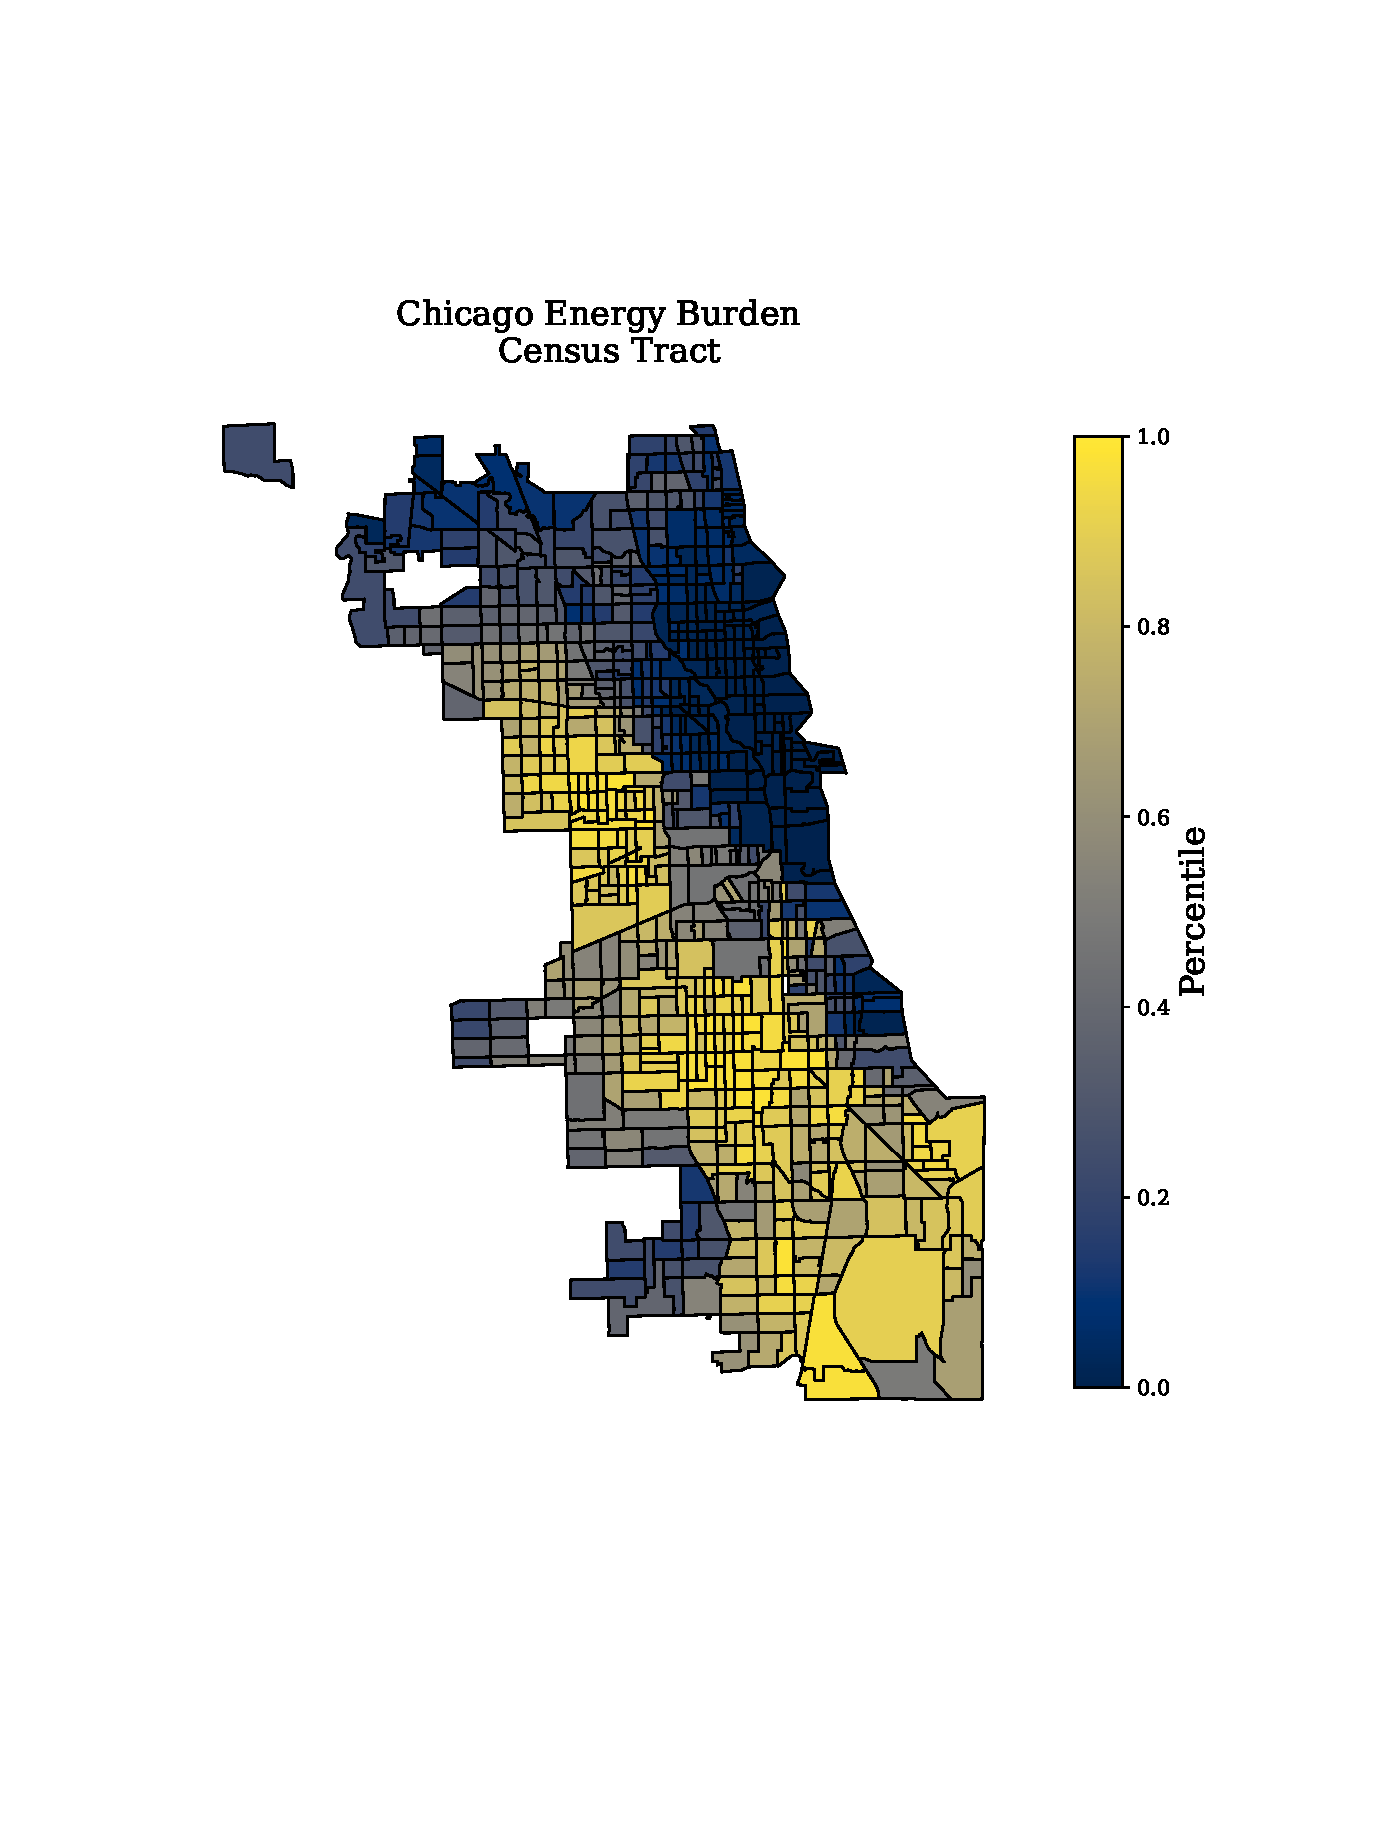
\includegraphics[trim=0 200 0 120, clip, width=\columnwidth]{energy_burden}
      % \vspace*{-3cm}
      \caption{Energy burden throughout Chicago as a percentile. A region in the zeroth
      percentile has the least energy burden and a region in the 100th percentile has
      more energy burden than any other region.}
      \label{fig:eb}
    \end{center}
\end{figure}

\subsubsection{Tree Canopy}

Urban tree cover effectively mitigates land surface temperatures in cities
\cite{loughner_roles_2012, schwaab_role_2021, mcdonald_tree_2021}. Tree canopy
reduces temperature by preventing ground heat storage through shade and encouraging
evapotranspiration \cite{mcdonald_tree_2021}. Thus, areas with greater tree cover
are less vulnerable heat waves. Figure \ref{fig:tree_census} shows the distribution
of trees in Chicago from the Morton Arboretum Tree Census \cite{kua_chicago_2020}.

\begin{figure}[H]
    \begin{center}
      \includegraphics[trim=0 200 0 120, clip, width=\columnwidth]{tree_canopy}
      % \vspace*{-3cm}
      \caption{Distribution of trees in Chicago by percentile. A region in the zeroth
      percentile has the least tree canopy and a region in the 100th percentile has
      more tree cover than any other region.}
      \label{fig:tree_census}
    \end{center}
\end{figure}

\subsubsection{Crime Rate}

An ethnographic study of the 1995 Chicago heat wave found that income level was
not the only predictor of heat wave mortalities as communities with similar income
levels had different heat wave outcomes. Some of this difference was explained by
crime rate as heat wave victims elected to keep their windows and doors shut out
of fears of crime \cite{klinenberg_heat_2003}.  This fear is prevalent among
the elderly whose age is an additional vulnerability \cite{gronlund_racial_2014}.
We filtered out crimes whose primary descriptions included ``gambling,''
``non-criminal,'' or ``interference with public officer.'' Otherwise, we did not
distinguish between violent crimes and ``non-violent'' ones.
Figure \ref{fig:crime} shows a heatmap of the crime locations in Chicago for 2021.

\begin{figure}[H]
    \begin{center}
      % \vspace*{-1cm}
      \includegraphics[trim=0 200 0 100, clip, width=\columnwidth]{crime_map}
      % \vspace*{-3cm}
      \caption{Map of crime locations in Chicago from 2021.}
      \label{fig:crime}
    \end{center}
\end{figure}

\subsection{Data Processing}
The data were prepared by first normalizing using the infinity norm,
\begin{eqnarray}
  L^{\infty} = \textnormal{max}\left(\mathbf{X}\right),
\end{eqnarray}
of each dataset to ensure all values are between zero and unity. Then, all
mitigating values, as identified in Table \ref{tab:data}, are subtracted from unity.
For example, this process negates the percentage of area covered by tree canopy
into  the percentage of community area not covered by tree canopy. Doing this
facilitates simple interpretation and identification of high-risk areas without
invoking complicated weighting schemes.

\subsection{Hierarchical Clustering}
In this study, we use hierarchical clustering to identify regions of similar risk.
Hierarchical clustering maximizes the similarity among samples within a cluster,
while simultaneously maximizing the differences across clusters \cite{karypis_chameleon_1999,
kotzur_impact_2018,rodriguez_clustering_2019}. The fundamental algorithm is
\begin{enumerate}
  \item set each sample as its own cluster;
  \item determine the ``mean'' sample of each cluster;
  \item measure the Euclidean distance between each cluster;
  \item Merge the two clusters with the minimum distance;
  \item check if the number of clusters is greater than the desired number;
  \item stop if the desired number of clusters is exceeded, otherwise, return
  to step 2.
\end{enumerate}

This algorithm is implemented in the Python library Scikit-learn \cite{scikit-learn}
which was used throughout this work.
Finally, we prioritize the clusters according to the $L^1$-norm of each cluster's
mean sample, where
\begin{eqnarray}
  L^1 = \|\mathbf{X}\|_1 = \sum_{i}^N x_i.
\end{eqnarray}
This gives each cluster a ``score'' between zero and the number of data points
used in the analysis.
